\documentclass[a4paper, smallheadings,english]{scrartcl}

% enable mutated vowls
\usepackage[utf8]{inputenc}

% vector fonts
\usepackage[T1]{fontenc}
% }}}

% {{{ include packages: math, url, fancyhdr
% break up syllables
\usepackage[english,ngerman]{babel}

% add notes to the doc
\usepackage{marginnote}

% use math
\usepackage{amsmath, amssymb, amsfonts}

% add graphics
\usepackage{lscape, tikz, graphicx}
\usetikzlibrary{backgrounds}

% display urls, code
\usepackage{url, listings}
\lstset{breaklines,commentstyle=\small\ttfamily,basicstyle=\scriptsize\ttfamily}

% enable custom headings
\usepackage{fancyhdr,lastpage,enumerate}
\renewcommand{\labelenumi}{(\roman{enumi})}
% }}}

%{{{ custom headings
%\pagestyle{plain}
% how do I refer to the author, chapter, etc?

\pagestyle{fancy}
\fancyhead[LO]{\Title} %Kopfzeile links
\fancyhead[LE]{\leftmark\rightmark} %Kopfzeile links
\fancyhead[R]{\Author} %Kopfzeile rechts
\fancyfoot[C]{\footnotesize \thepage\ of \pageref{LastPage}}
\fancypagestyle{firststyle}
{
    \renewcommand{\headrulewidth}{0pt}
    \fancyhf{}
    \fancyfoot[C]{\footnotesize \thepage\ of \pageref{LastPage}}
}
% }}}

\newcommand{\Author}{Jiannan Guo - ICT-Innovation\\Niklas Semmler - ICT-Innovation}
\newcommand{\Title}{Network Management Project}
\newcommand{\note}[1]{\marginnote{\textit{\textbf{#1}} }}
\newcommand{\corr}[2]{\marginnote{\textcolor{red}{#1} }}

\begin{document}
% {{{ Header
\title{\Title}
\author{\Author}
\date{\today}
\maketitle
% }}}
\thispagestyle{firststyle}
\section{Task I}
\begin{lstlisting}[caption={inspired by \cite{stadler2012protocols}}, numbers=left, frame=single]
messages:
(new, n)
(fail, n)
(update, n; l; p; a)
(localvar, x)

procedure GAP( )
    T := empty table;
    if v = root then
        addEntry(root, parent, -1, undef);
        addEntry(root, self, 0, undef);
    else
        addEntry(v, self, undef, undef);
    end if
    vector := updateVector();
    send (update, v; vector) to all neighbors;
    A.initiate();
    while true do
        read message;
        switch (message)
            case (new, from):
                addEntry(from, peer, undef, undef);
                send (update, v; vector) to from;
            case (fail, from):
                removeEntry(from);
            case (localvar, x):
                empty;
            case (update, from; level; parent; aggregate):
                updateEntry(from; level; parent; aggregate);
        end switch
        restoreTableInvariant();
        A.aggregate(); if (v =root) then A.global();
        newvector := updateVector();
        if newvector 6 = vector then
            send (update, v; newvector) to all neighbors;
            vector := newvector;
        end if
    end while
    end procedure
\end{lstlisting}
\begin{lstlisting}[caption={inspired by \cite{stadler2012protocols}}, numbers=left, frame=single]
messages:
(ResponseTimeArriveMessage, responseTime)
(UpdateVector, neighbor)
(TimeOut, responseTime)

help functions:
A.aggregate_local
A.aggregate_sub_tree
A.value
A.global
send_to_self
send_to_neighbors
send_to_parent
find_parent

procedure GAP( )
    DELAY = # fixed time window
    Neighbors := empty;
    ResponseTimes := empty;

    if v = root then
        level = 0
        parent = 0
    else
        level = INF
        parent = INF
    end if

    A.initiate()
    while true do
        read message;
        switch (message)
            case (ResponseTimeArriveMessage, responseTime)
                ResponseTimes.add(responseTime)
                # to keep only a set of responseTimes in cache
                send_to_self(DELAY, TimeOut(responseTime))
                A.aggregate_local(ResponseTimes)
                A.aggregate_sub_tree(Neighbors)
            case (UpdateVector, neighbor):
                Neighbors.add(neighbor) 
                (newParent, newLevel) = find_new_parent(Neighbors)
                A.aggregate_sub_tree(Neighbors)
                if level != newLevel then
                    level = newLevel
                    parent = newParent
                    send_to_neighbors(Neighbors, level, parent, A.value())
                    continue
                end if
            # to keep only a set of responseTimes in cache
            case (TimeOut, responseTime):
                responses.remove(responseTime)
                A.aggregate_local_value(ResponseTimes)
                A.aggregate_sub_tree(Neighbors)
        end switch
        if (v =root) then A.global()

        # TODO: reformulate below!!!
        newvector := updateVector();
        if newvector != vector then
            send (update, newvector) to all neighbors;
            vector := newvector;
        end if
        send_to_parent(Neighbors, A.value)
    end while
    end procedure
\end{lstlisting}

\begin{figure}[h!]
    \begin{center}
        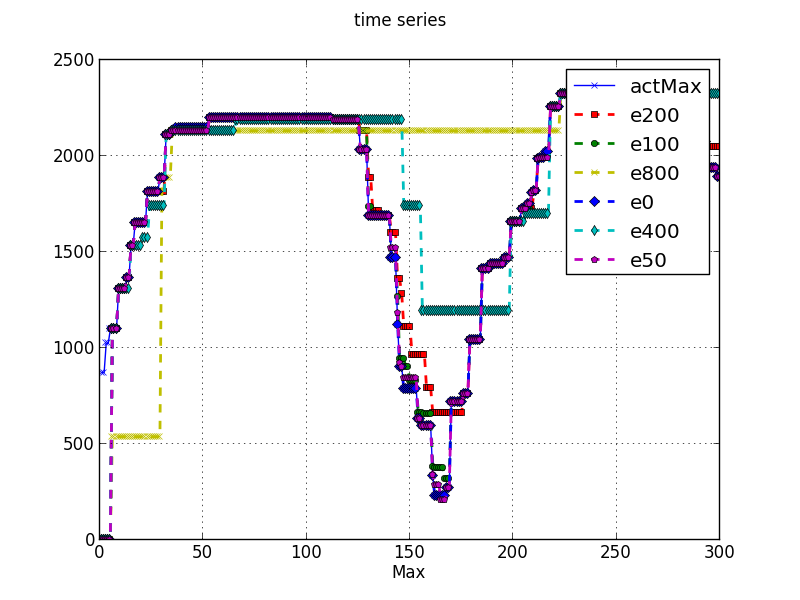
\includegraphics[scale=0.7]{plots/time_series}
    \end{center}
    \caption{Time series plot}
    \label{fig:ts}
\end{figure}
\begin{figure}[h!]
    \begin{center}
        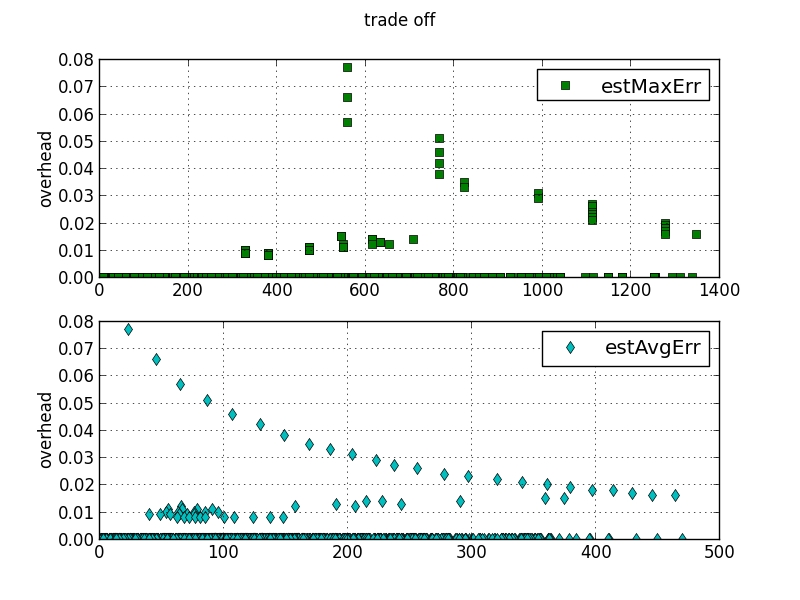
\includegraphics[scale=0.7]{plots/trade_off}
    \end{center}
    \caption{Trade off plot}
    \label{fig:to}
\end{figure}
\begin{figure}[h!]
    \begin{center}
        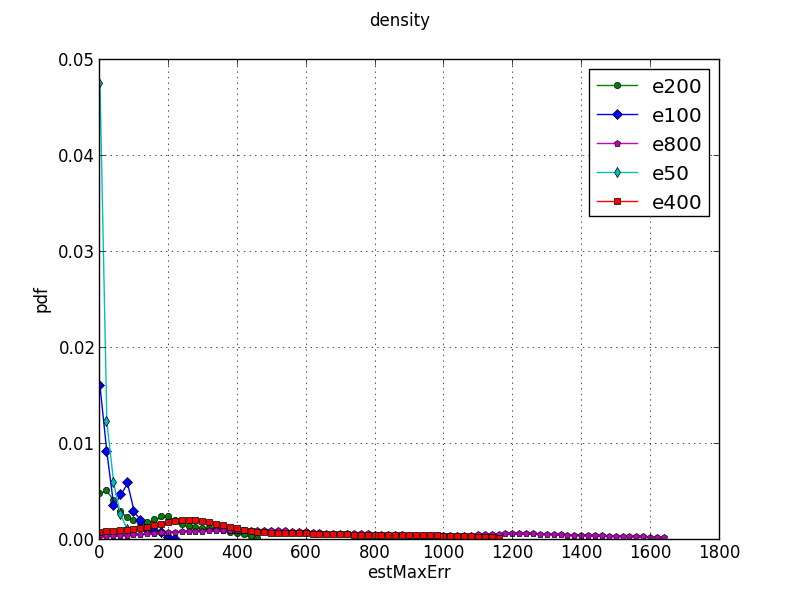
\includegraphics[scale=0.7]{plots/pdf_of_error}
    \end{center}
    \caption{PDF plot}
    \label{fig:pdf}
\end{figure}



\begin{itemize}
    \item compare performance for $R_1, R_2$
    \begin{itemize}
        \item time series of f~(t) and f(t) for r = \{ 0.2, 0.4, 0.8 \} amd \{$R_1$, $R_2$\} from the first 5 min
        \item trade off plot for $R_1, R_2$
        \item density plot for r = \{ 0.2, 0.4, 0.8 \} and \{$R_1$, $R_2$\}
    \end{itemize}
\end{itemize}

\section{Task II}
\begin{itemize}
    \item pseudo code!
    \item implementation details
    \item compare performance for $R_1, R_2$
    \begin{itemize}
        \item time series of f~(t) and f(t) for r = \{ 0.2, 0.1, 0.05, 0.025, \} amd \{$R_1$, $R_2$\} from the first 5 min
        \item trade off plot for $R_1, R_2$
        \item density plot for r = \{ 0.1, 0.05, 0.025 \} and \{$R_1$, $R_2$\}
    \end{itemize}
\end{itemize}

\section{Task III}
\begin{itemize}
    \item pseudo code!
    \item implementation details
    \item compare performance for $R_1, R_2$
    \begin{itemize}
        \item time series of f~(t) and f(t) for r = \{ 0.2, 0.1, 0.05, 0.025, \} amd \{$R_1$, $R_2$\} from the first 5 min
        \item trade off plot for $R_1, R_2$
        \item density plot for r = \{ 0.1, 0.05, 0.025 \} and \{$R_1$, $R_2$\}
    \end{itemize}
\end{itemize}

\section{Summary}
\begin{itemize}
    \item Compare TaskI, II, III
    \item Compare $R_1, R_2$ globally
\end{itemize}
\bibliographystyle{ieeetr}
\bibliography{report}

\end{document}
